% ============================================================
% DSC 40B — Homework Template
% Usage: compile with pdflatex (or latexmk -pdf)
% Fill in \name and \hwnum below. Date auto-fills via \today.
% ============================================================
\documentclass[11pt]{article}

% ---------- Packages ----------
\usepackage[margin=1in]{geometry}
\usepackage{amsmath, amssymb, amsthm}   % math environments, symbols, proofs
\usepackage{mathtools}                  % \coloneqq, better \DeclarePairedDelimiter
\usepackage{enumitem}                   % control over list labels/spacing
\usepackage{tikz}                       % graph drawing
\usetikzlibrary{positioning, arrows.meta} % relative node placement, arrow tips
\usepackage{fancyhdr}                   % header/footer
\usepackage{hyperref}                   % clickable links in sources list
\usepackage{listings}                   % code listings
\usepackage{xcolor}                     % colors for syntax highlighting

% ---------- Python code style ----------
% Usage: \begin{lstlisting} ... \end{lstlisting}
% Continue numbering from line N: \begin{lstlisting}[firstnumber=N]
\lstdefinestyle{pystyle}{
  language=Python,
  numbers=left,                 % line numbers
  numberstyle=\tiny\color{gray},
  basicstyle=\ttfamily\small,
  keywordstyle=\color{blue},
  commentstyle=\color{gray}\itshape,
  stringstyle=\color{teal},
  frame=single,                 % box around code; remove if unwanted
  breaklines=true,
  showstringspaces=false,
  tabsize=4
}
\lstset{style=pystyle}

% ---------- Student info (EDIT THESE) ----------
\newcommand{\name}{FirstName LastName}
\newcommand{\hwnum}{X}                  % homework number
\newcommand{\course}{DSC 40B}           % course code
\newcommand{\term}{Summer 2026}         % term

% ---------- Footer (page numbers only; header is the handout box) ----------
\pagestyle{fancy}
\fancyhf{}
\renewcommand{\headrulewidth}{0pt}
\cfoot{\thepage}

% ---------- Handout box ----------
% \handout{course}{term}{left-italic}{right-italic}{center-title}
\newcommand{\handout}[5]{
  \noindent
  \begin{center}
  \framebox{
    \vbox{
      \hbox to 5.78in { {\bf #1} \hfill #2 }
      \vspace{4mm}
      \hbox to 5.78in { {\Large \hfill #5  \hfill} }
      \vspace{2mm}
      \hbox to 5.78in { {\it #3 \hfill #4} }
    }
  }
  \end{center}
  \vspace*{4mm}
}

% ============================================================
% COURSE NOTATION MACROS
% Use these instead of typing raw commands each time.
% ============================================================

% --- Asymptotic notation ---
\newcommand{\bigO}[1]{O\!\left(#1\right)}          % \bigO{n \log n}  ->  O(n log n)
\newcommand{\bigTheta}[1]{\Theta\!\left(#1\right)} % \bigTheta{n^2}   ->  Θ(n²)
\newcommand{\bigOmega}[1]{\Omega\!\left(#1\right)} % \bigOmega{n}     ->  Ω(n)

% --- Common sets ---
\newcommand{\R}{\mathbb{R}}
\newcommand{\N}{\mathbb{N}}
\newcommand{\Z}{\mathbb{Z}}

% --- Floor / ceiling ---
\DeclarePairedDelimiter{\floor}{\lfloor}{\rfloor}  % \floor{n/2}
\DeclarePairedDelimiter{\ceil}{\lceil}{\rceil}     % \ceil{\log n}

% --- Absolute value / set cardinality ---
\DeclarePairedDelimiter{\abs}{\lvert}{\rvert}      % \abs{V}, \abs{E}

% --- Problem environment: \begin{problem}{1} ... \end{problem} ---
\newcounter{problem}
\newenvironment{problem}[1]{%
  \setcounter{problem}{#1}%
  \section*{Problem \theproblem}%
}{\bigskip}

% Optional: theorem-style environments if a proof is required
\newtheorem{claim}{Claim}

% ============================================================
\begin{document}

\handout{\course}{\term}{\name}{\today}{Homework \hwnum}

% ---------- Sources ----------
\section*{Sources}
\begin{itemize}[nosep]
  \item Course notes: \url{https://dsc40b.com/materials/default/notes/book.pdf}
  \item % add collaborators / other sources here
\end{itemize}

% ============================================================
% NOTATION REFERENCE (delete this block in your submission;
% it exists to show what each macro renders as)
% ============================================================
\section*{Notation Reference}

\textbf{Asymptotics:}
\[
  f(n) = \bigO{n \log n}, \quad
  f(n) = \bigTheta{n^2}, \quad
  f(n) = \bigOmega{n}, \quad
\]

\textbf{Relational / logic symbols:}
\[
  \leq \quad \geq \quad \neq \quad \approx \quad \ll \quad \gg \quad
  \implies \quad \iff \quad \forall \quad \exists \quad \in \quad \subseteq
\]

\textbf{Recurrences} (use \texttt{cases} for base/recursive case):
\[
  T(n) =
  \begin{cases}
    \bigTheta{1} & n \leq 1 \\
    2\,T\!\left(\floor{n/2}\right) + \bigTheta{n} & n > 1
  \end{cases}
\]

\textbf{Absolute value (or length in graph theory)}
\[
   \abs{V} = n, \quad \abs{E} = m
\]

\textbf{Graph example} (TikZ; \texttt{->} on the tikzpicture makes it directed,
remove for undirected; edge labels are weights):

\begin{center}
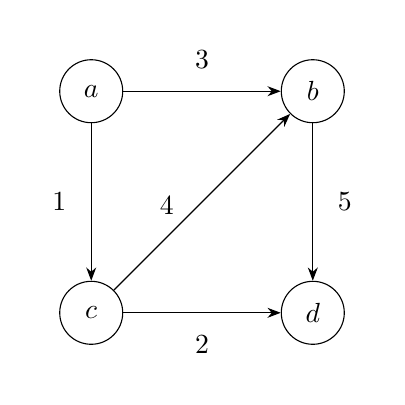
\begin{tikzpicture}[
  node distance=2cm,
  every node/.style={circle, draw, minimum size=8mm},
  ->, >={Stealth}                % directed edges; delete this line for undirected
]
  % --- nodes: \node (id) [position] {label}; ---
  \node (a) {$a$};
  \node (b) [right=of a] {$b$};
  \node (c) [below=of a] {$c$};
  \node (d) [right=of c] {$d$};

  % --- edges: \draw (from) -- node[...]{weight} (to); ---
  \draw (a) -- node[draw=none, above] {3} (b);
  \draw (a) -- node[draw=none, left]  {1} (c);
  \draw (c) -- node[draw=none, below] {2} (d);
  \draw (b) -- node[draw=none, right] {5} (d);
  \draw (c) -- node[draw=none, above, pos=0.3] {4} (b);
\end{tikzpicture}
\end{center}



% ============================================================
% PROBLEMS
% ============================================================
\newpage 
\begin{problem}{1}
Solution:
\begin{lstlisting}
def linear_search(arr, target):
    for i in range(len(arr)):
        if arr[i] == target:
            return i
    return -1
\end{lstlisting}
\end{problem}

\begin{problem}{2}
% your solution here
\end{problem}

\begin{problem}{3}
% your solution here
\end{problem}

% Add more \begin{problem}{N} ... \end{problem} blocks as needed.

\end{document}